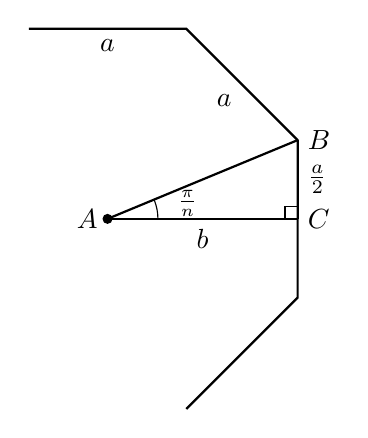
\begin{tikzpicture}[scale=0.8]
  \def \a {2.5}
  \def \b {(\a/2 + \a/sqrt(2))}

  \coordinate (A) at (0, 0);
  \coordinate (B) at ({\b}, {\a/2});
  \coordinate (C) at ({\b}, 0);

  \draw[thick] ({\b - \a * cos(45) - \a}, {\a/2 + \a * sin(45)}) 
    -- ({\b - \a * cos(45)}, {\a/2 + \a * sin(45)}) node[midway, anchor=north] {$a$}
    -- (B) node[midway, anchor=north east] {$a$}
    -- ({\b}, -{\a/2})
    -- ({\b - \a * cos(45)}, {-\a/2 - \a * sin(45)});

  \draw[thick] (A) -- (B) node[anchor=west] {$B$};
  \draw[thick] (A) -- (C) node[midway, anchor=north] {$b$} 
                          node[anchor=west] {$C$};
  \draw[thick] (B) -- (C) node[midway, anchor=west] {$\frac{a}{2}$};
 
  \draw ({\b - 0.2}, 0) -- ({\b - 0.2}, 0.2) -- ({\b}, 0.2); % right angle sign
  \draw (0.8, 0) arc (0:{atan((\a/2)/\b)}:0.8) 
    node[midway, anchor=west, xshift=4, yshift=2] {\small$\frac{\pi}{n}$};
  
  \filldraw[black] (A) circle (2pt)
    node[anchor=east] {$A$};
\end{tikzpicture}
